% Options for packages loaded elsewhere
\PassOptionsToPackage{unicode}{hyperref}
\PassOptionsToPackage{hyphens}{url}
%
\documentclass[
  letterpaper,
  oneside,
  open=any]{scrbook}

\usepackage{amsmath,amssymb}
\usepackage{iftex}
\ifPDFTeX
  \usepackage[T1]{fontenc}
  \usepackage[utf8]{inputenc}
  \usepackage{textcomp} % provide euro and other symbols
\else % if luatex or xetex
  \usepackage{unicode-math}
  \defaultfontfeatures{Scale=MatchLowercase}
  \defaultfontfeatures[\rmfamily]{Ligatures=TeX,Scale=1}
\fi
\usepackage{lmodern}
\ifPDFTeX\else  
    % xetex/luatex font selection
\fi
% Use upquote if available, for straight quotes in verbatim environments
\IfFileExists{upquote.sty}{\usepackage{upquote}}{}
\IfFileExists{microtype.sty}{% use microtype if available
  \usepackage[]{microtype}
  \UseMicrotypeSet[protrusion]{basicmath} % disable protrusion for tt fonts
}{}
\makeatletter
\@ifundefined{KOMAClassName}{% if non-KOMA class
  \IfFileExists{parskip.sty}{%
    \usepackage{parskip}
  }{% else
    \setlength{\parindent}{0pt}
    \setlength{\parskip}{6pt plus 2pt minus 1pt}}
}{% if KOMA class
  \KOMAoptions{parskip=half}}
\makeatother
\usepackage{xcolor}
\setlength{\emergencystretch}{3em} % prevent overfull lines
\setcounter{secnumdepth}{5}
% Make \paragraph and \subparagraph free-standing
\ifx\paragraph\undefined\else
  \let\oldparagraph\paragraph
  \renewcommand{\paragraph}[1]{\oldparagraph{#1}\mbox{}}
\fi
\ifx\subparagraph\undefined\else
  \let\oldsubparagraph\subparagraph
  \renewcommand{\subparagraph}[1]{\oldsubparagraph{#1}\mbox{}}
\fi

\providecommand{\tightlist}{%
  \setlength{\itemsep}{0pt}\setlength{\parskip}{0pt}}\usepackage{longtable,booktabs,array}
\usepackage{calc} % for calculating minipage widths
% Correct order of tables after \paragraph or \subparagraph
\usepackage{etoolbox}
\makeatletter
\patchcmd\longtable{\par}{\if@noskipsec\mbox{}\fi\par}{}{}
\makeatother
% Allow footnotes in longtable head/foot
\IfFileExists{footnotehyper.sty}{\usepackage{footnotehyper}}{\usepackage{footnote}}
\makesavenoteenv{longtable}
\usepackage{graphicx}
\makeatletter
\def\maxwidth{\ifdim\Gin@nat@width>\linewidth\linewidth\else\Gin@nat@width\fi}
\def\maxheight{\ifdim\Gin@nat@height>\textheight\textheight\else\Gin@nat@height\fi}
\makeatother
% Scale images if necessary, so that they will not overflow the page
% margins by default, and it is still possible to overwrite the defaults
% using explicit options in \includegraphics[width, height, ...]{}
\setkeys{Gin}{width=\maxwidth,height=\maxheight,keepaspectratio}
% Set default figure placement to htbp
\makeatletter
\def\fps@figure{htbp}
\makeatother
% definitions for citeproc citations
\NewDocumentCommand\citeproctext{}{}
\NewDocumentCommand\citeproc{mm}{%
  \begingroup\def\citeproctext{#2}\cite{#1}\endgroup}
\makeatletter
 % allow citations to break across lines
 \let\@cite@ofmt\@firstofone
 % avoid brackets around text for \cite:
 \def\@biblabel#1{}
 \def\@cite#1#2{{#1\if@tempswa , #2\fi}}
\makeatother
\newlength{\cslhangindent}
\setlength{\cslhangindent}{1.5em}
\newlength{\csllabelwidth}
\setlength{\csllabelwidth}{3em}
\newenvironment{CSLReferences}[2] % #1 hanging-indent, #2 entry-spacing
 {\begin{list}{}{%
  \setlength{\itemindent}{0pt}
  \setlength{\leftmargin}{0pt}
  \setlength{\parsep}{0pt}
  % turn on hanging indent if param 1 is 1
  \ifodd #1
   \setlength{\leftmargin}{\cslhangindent}
   \setlength{\itemindent}{-1\cslhangindent}
  \fi
  % set entry spacing
  \setlength{\itemsep}{#2\baselineskip}}}
 {\end{list}}
\usepackage{calc}
\newcommand{\CSLBlock}[1]{\hfill\break\parbox[t]{\linewidth}{\strut\ignorespaces#1\strut}}
\newcommand{\CSLLeftMargin}[1]{\parbox[t]{\csllabelwidth}{\strut#1\strut}}
\newcommand{\CSLRightInline}[1]{\parbox[t]{\linewidth - \csllabelwidth}{\strut#1\strut}}
\newcommand{\CSLIndent}[1]{\hspace{\cslhangindent}#1}

\usepackage[default]{opensans}
\fontseries{lc}\selectfont
\usepackage{caption}
\captionsetup[figure]{font=footnotesize, justification=justified, format=plain, singlelinecheck=false, labelformat=simple}
\makeatletter
\@ifpackageloaded{tcolorbox}{}{\usepackage[skins,breakable]{tcolorbox}}
\@ifpackageloaded{fontawesome5}{}{\usepackage{fontawesome5}}
\definecolor{quarto-callout-color}{HTML}{909090}
\definecolor{quarto-callout-note-color}{HTML}{0758E5}
\definecolor{quarto-callout-important-color}{HTML}{CC1914}
\definecolor{quarto-callout-warning-color}{HTML}{EB9113}
\definecolor{quarto-callout-tip-color}{HTML}{00A047}
\definecolor{quarto-callout-caution-color}{HTML}{FC5300}
\definecolor{quarto-callout-color-frame}{HTML}{acacac}
\definecolor{quarto-callout-note-color-frame}{HTML}{4582ec}
\definecolor{quarto-callout-important-color-frame}{HTML}{d9534f}
\definecolor{quarto-callout-warning-color-frame}{HTML}{f0ad4e}
\definecolor{quarto-callout-tip-color-frame}{HTML}{02b875}
\definecolor{quarto-callout-caution-color-frame}{HTML}{fd7e14}
\makeatother
\makeatletter
\@ifpackageloaded{bookmark}{}{\usepackage{bookmark}}
\makeatother
\makeatletter
\@ifpackageloaded{caption}{}{\usepackage{caption}}
\AtBeginDocument{%
\ifdefined\contentsname
  \renewcommand*\contentsname{Table of contents}
\else
  \newcommand\contentsname{Table of contents}
\fi
\ifdefined\listfigurename
  \renewcommand*\listfigurename{List of Figures}
\else
  \newcommand\listfigurename{List of Figures}
\fi
\ifdefined\listtablename
  \renewcommand*\listtablename{List of Tables}
\else
  \newcommand\listtablename{List of Tables}
\fi
\ifdefined\figurename
  \renewcommand*\figurename{Figure}
\else
  \newcommand\figurename{Figure}
\fi
\ifdefined\tablename
  \renewcommand*\tablename{Table}
\else
  \newcommand\tablename{Table}
\fi
}
\@ifpackageloaded{float}{}{\usepackage{float}}
\floatstyle{ruled}
\@ifundefined{c@chapter}{\newfloat{codelisting}{h}{lop}}{\newfloat{codelisting}{h}{lop}[chapter]}
\floatname{codelisting}{Listing}
\newcommand*\listoflistings{\listof{codelisting}{List of Listings}}
\makeatother
\makeatletter
\makeatother
\makeatletter
\@ifpackageloaded{caption}{}{\usepackage{caption}}
\@ifpackageloaded{subcaption}{}{\usepackage{subcaption}}
\makeatother

\usepackage{hyphenat}
\usepackage{ifthen}
\usepackage{calc}
\usepackage{calculator}

\usepackage{graphicx}
\usepackage{wallpaper}

\usepackage{geometry}

\usepackage{graphicx}
\usepackage{geometry}
\usepackage{afterpage}
\usepackage{tikz}
\usetikzlibrary{calc}
\usetikzlibrary{fadings}
\usepackage[pagecolor=none]{pagecolor}


% Set the titlepage font families







% Set the coverpage font families

\ifLuaTeX
  \usepackage{selnolig}  % disable illegal ligatures
\fi
\usepackage{bookmark}

\IfFileExists{xurl.sty}{\usepackage{xurl}}{} % add URL line breaks if available
\urlstyle{same} % disable monospaced font for URLs
\hypersetup{
  pdftitle={{[}Template{]} Ecosystem Status Report},
  pdfauthor={Gulf of America Integrated Ecosystem Assessment Program},
  hidelinks,
  pdfcreator={LaTeX via pandoc}}

\title{{[}Template{]} Ecosystem Status Report}
\author{Gulf of America Integrated Ecosystem Assessment Program}
\date{2025-09-08}

\begin{document}
%%%%% begin titlepage extension code

  \begin{frontmatter}

\begin{titlepage}
% This is a combination of Pandoc templating and LaTeX
% Pandoc templating https://pandoc.org/MANUAL.html#templates
% See the README for help

\thispagestyle{empty}

\newgeometry{top=-100in}

% Page color

\newcommand{\coverauthorstyle}[1]{{\fontsize{20}{24.0}\selectfont
{#1}}}

\begin{tikzpicture}[remember picture, overlay, inner sep=0pt, outer sep=0pt]

\tikzfading[name=fadeout, inner color=transparent!0,outer color=transparent!100]
\tikzfading[name=fadein, inner color=transparent!100,outer color=transparent!0]
\node[anchor=south west, rotate=0.0, opacity=1.0] at ($(current page.south west)+(0pt, 8.75in)$) {

\includegraphics[width=\paperwidth, keepaspectratio]{report/images/cover-header-2.png}};

% Title
\newcommand{\titlelocationleft}{2.3in}
\newcommand{\titlelocationbottom}{7in}
\newcommand{\titlealign}{left}

\begin{scope}{%
\fontsize{30}{36.0}\selectfont
\node[anchor=north
west, align=left, rotate=0] (Title1) at ($(current page.south west)+(\titlelocationleft,\titlelocationbottom)$)  [text width = 5in]  {\textcolor{black}{\bfseries{\nohyphens{{[}Template{]}
Ecosystem Status Report}}}};
}
\end{scope}

% Author
\newcommand{\authorlocationleft}{2.3in}
\newcommand{\authorlocationbottom}{5in}
\newcommand{\authoralign}{left}

\begin{scope}
{%
\fontsize{20}{24.0}\selectfont
\node[anchor=north
west, align=left, rotate=0] (Author1) at ($(current page.south west)+(\authorlocationleft,\authorlocationbottom)$)  [text width = 5in]  {\coverauthorstyle{Gulf
of America Integrated Ecosystem Assessment Program\\}};
}
\end{scope}

% Header
\newcommand{\headerlocationleft}{2.3in}
\newcommand{\headerlocationbottom}{9.8in}
\newcommand{\headerlocationalign}{left}

\begin{scope}
{%
\fontsize{16}{19.2}\selectfont
 \node[anchor=north west, align=left, rotate=0] (Header1) at %
($(current page.south west)+(\headerlocationleft,\headerlocationbottom)$)  [text width = 5in]  {\textcolor{white}{\nohyphens{NOAA
Technical Memorandum NMFS-XXX-\#\#}}};
}
\end{scope}

% Footer
\newcommand{\footerlocationleft}{6in}
\newcommand{\footerlocationbottom}{0.1\paperheight}
\newcommand{\footerlocationalign}{left}

\begin{scope}
{%
\fontsize{8}{9.6}\selectfont
 \node[anchor=north west, align=left, rotate=0] (Footer1) at %
($(current page.south west)+(\footerlocationleft,\footerlocationbottom)$)  [text width = 2.5in]  {{\nohyphens{U.S.
DEPARTMENT OF COMMERCE\\
\strut \\
National Oceanic and Atmospheric Administration\\
National Marine Fisheries Service\\
Northwest Fisheries Science Center}}};
}
\end{scope}

% Date
\newcommand{\datelocationleft}{6in}
\newcommand{\datelocationbottom}{2in}
\newcommand{\datelocationalign}{left}

\begin{scope}
{%
\fontsize{20}{24.0}\selectfont
 \node[anchor=north west, align=left, rotate=0] (Date1) at %
($(current page.south west)+(\datelocationleft,\datelocationbottom)$)  [text width = 2.5in]  {{\nohyphens{2025-09-08}}};
}
\end{scope}

\end{tikzpicture}
\clearpage
\restoregeometry
%%% TITLE PAGE START

% Set up alignment commands
%Page
\newcommand{\titlepagepagealign}{
\ifthenelse{\equal{left}{right}}{\raggedleft}{}
\ifthenelse{\equal{left}{center}}{\centering}{}
\ifthenelse{\equal{left}{left}}{\raggedright}{}
}
%% Titles
\newcommand{\titlepagetitlealign}{
\ifthenelse{\equal{left}{right}}{\raggedleft}{}
\ifthenelse{\equal{left}{center}}{\centering}{}
\ifthenelse{\equal{left}{left}}{\raggedright}{}
\ifthenelse{\equal{left}{spread}}{\makebox[\linewidth][s]}{}
}


\newcommand{\titleandsubtitle}{
% Title and subtitle
{\fontsize{30}{36.0}\selectfont
\textcolor{black}{\bfseries{\nohyphens{{[}Template{]} Ecosystem Status
Report}}}\par
}%
}
\newcommand{\titlepagetitleblock}{
\titleandsubtitle
}

\newcommand{\authorstyle}[1]{{\fontsize{20}{24.0}\selectfont
#1}}

\newcommand{\affiliationstyle}[1]{{#1}}

\newcommand{\titlepageauthorblock}{
{\authorstyle{\nohyphens{Gulf of America Integrated Ecosystem Assessment
Program}{\textsuperscript{1}}}}}

\newcommand{\titlepageaffiliationblock}{
\hangindent=1em
\hangafter=1
{\affiliationstyle{
{1}.~NOAA Fisheres,~Southeast Fisheries Science Center


\vspace{1\baselineskip} 
}}
}
\newcommand{\headerstyled}{%
{}
}
\newcommand{\footerstyled}{%
{}
}
\newcommand{\datestyled}{%
{2025-09-08}
}


\newcommand{\titlepageheaderblock}{\headerstyled}

\newcommand{\titlepagefooterblock}{
\footerstyled
}

\newcommand{\titlepagedateblock}{
\datestyled
}

%set up blocks so user can specify order
\newcommand{\titleblock}{{\titlepagetitlealign

{\titlepagetitleblock}
}

\vspace{4\baselineskip}
}

\newcommand{\authorblock}{{\titlepageauthorblock}

\vspace{2\baselineskip}
}

\newcommand{\affiliationblock}{{\titlepageaffiliationblock}

\vspace{2\baselineskip}
}

\newcommand{\logoblock}{}

\newcommand{\footerblock}{}

\newcommand{\dateblock}{{\titlepagedateblock}

\vspace{0pt}
}

\newcommand{\headerblock}{}
\newgeometry{top=3in,bottom=1in,right=1in,left=1.75in}
% background image
\newlength{\bgimagesize}
\setlength{\bgimagesize}{0.75\paperwidth}
\LENGTHDIVIDE{\bgimagesize}{\paperwidth}{\theRatio} % from calculator pkg
\ThisULCornerWallPaper{\theRatio}{report/images/corner-image.png}

\thispagestyle{empty} % no page numbers on titlepages


\newcommand{\vrulecode}{\textcolor{black}{\rule{\vrulewidth}{\textheight}}}
\newlength{\vrulewidth}
\setlength{\vrulewidth}{0pt}
\newlength{\B}
\setlength{\B}{\ifdim\vrulewidth > 0pt 0.05\textwidth\else 0pt\fi}
\newlength{\minipagewidth}
\ifthenelse{\equal{left}{left} \OR \equal{left}{right} }
{% True case
\setlength{\minipagewidth}{\textwidth - \vrulewidth - \B - 0.1\textwidth}
}{
\setlength{\minipagewidth}{\textwidth - 2\vrulewidth - 2\B - 0.1\textwidth}
}
\ifthenelse{\equal{left}{left} \OR \equal{left}{leftright}}
{% True case
\raggedleft % needed for the minipage to work
\vrulecode
\hspace{\B}
}{%
\raggedright % else it is right only and width is not 0
}
% [position of box][box height][inner position]{width}
% [s] means stretch out vertically; assuming there is a vfill
\begin{minipage}[b][\textheight][s]{\minipagewidth}
\titlepagepagealign
\headerblock

\titleblock

\authorblock

\affiliationblock

\vfill

\logoblock

\footerblock
\par

\end{minipage}\ifthenelse{\equal{left}{right} \OR \equal{left}{leftright} }{
\hspace{\B}
\vrulecode}{}
\clearpage
\restoregeometry
%%% TITLE PAGE END
\end{titlepage}
\setcounter{page}{1}
\end{frontmatter}

%%%%% end titlepage extension code

\renewcommand*\contentsname{Table of contents}
{
\setcounter{tocdepth}{2}
\tableofcontents
}
\listoffigures
\mainmatter
\bookmarksetup{startatroot}

\chapter{Introduction}\label{introduction}

\begin{tcolorbox}[enhanced jigsaw, arc=.35mm, coltitle=black, leftrule=.75mm, titlerule=0mm, bottomrule=.15mm, colback=white, opacitybacktitle=0.6, colframe=quarto-callout-note-color-frame, opacityback=0, rightrule=.15mm, toprule=.15mm, bottomtitle=1mm, toptitle=1mm, title=\textcolor{quarto-callout-note-color}{\faInfo}\hspace{0.5em}{Editing this template page}, breakable, colbacktitle=quarto-callout-note-color!10!white, left=2mm]

Template text is pulled from the 2025 Caribbean Ecosystem Status Report.
Adjust accordingly.

\end{tcolorbox}

\section{About this report}\label{about-this-report}

The purpose of this report is to synthesize diverse information sources
to assist with implementation of ecosystem-based fisheries management in
the U.S. Caribbean region, which includes Puerto Rico and the U.S.
Virgin Islands (USVI). A suite of indicators that span physical,
biological, social and economic elements of the ecosystem are reported
with the goal of helping the Caribbean Fishery Management Council (CFMC)
and other resource managers measure progress toward fishery management
objectives. The report relies on both previously identified proposed
indicators and expert vetting to select a suite of indicators that best
address the fishery management plan (FMP) objectives for the U.S.
Caribbean. Information in this report is organized into two sections: 1)
tracking performance toward predefined fishery management objectives,
and 2) potential risks to meeting those fishery management objectives.

The first set of indicators can be used to consider progress toward
stated management objectives. Management objectives were gleaned from
the Island-based Fishery Management Plans and categorized into seven
groups: food production, socioeconomic health, equity, engagement and
participation, bycatch reduction, governance, and protection of
ecosystems. Each of these sections contains a selection of indicators
that can be used to better understand how well these respective
management objectives are being met. Note that for some indicators,
directionality can be associated with positive or negative progress
toward management objectives (e.g., increases in abundance of
economically important species is generally associated with improved
management). However for other indicators, directionality can be
considered neutral (e.g., proportion of diving trips, changes in
contribution to revenue), although changes in these indicators represent
important shifts in the fishing dynamics of which managers should be
aware. The risk indicator section quantifies major stressors (as
identified by stakeholders) that capture the potential risks to meeting
fishery management objectives. These indicators provide managers with an
understanding of the backdrop against which management is occurring.
Major changes in these indicators may be associated with decreased
effectiveness of fisheries management, if the influences of external
environmental or economic stressors are strong relative to influences
from adjustments in fishing activity.

This report was created in Quarto
(\url{https://github.com/quarto-dev/quarto-cli/}) using the NOAA Quarto
book template
(\hyperref[0]{https://github.com/nmfs-opensci/NOAA-quarto-book}). A
github repository houses all the indicator data and R code used to
compile the report
(\hyperref[0]{https://github.com/Gulf-IEA/Caribbean-ESR-2}).

\section{Indicator selection}\label{indicator-selection}

The CFMC's Science and Statistical Committee, as well as the region's
Ecosystem-Based Fishery Management Technical Advisory Panel (EBFM TAP),
recently completed a series of conceptual models linking key components
of the ecosystem and human activities related to fishing (Seara et al.
2024). This report used these conceptual models as a starting list of
proposed indicators and matched the indicators to address progress
toward FMP objectives when possible (Figure~\ref{fig-flowchart}).

\begin{figure}

\centering{

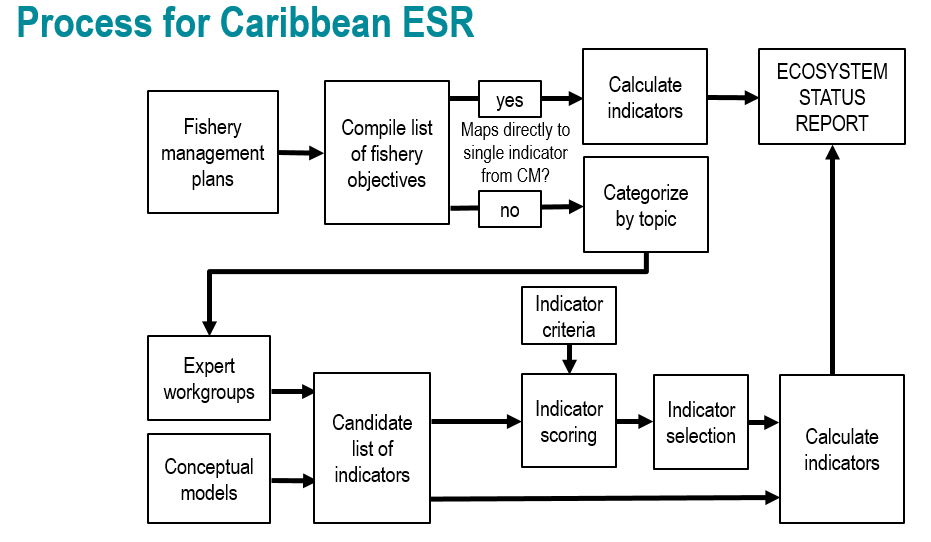
\includegraphics[width=5.36458in,height=\textheight]{figures/images/process_flow_chart.png}

}

\caption{\label{fig-flowchart}Process for selecting indicators for the
U.S. Caribbean Ecosystem Status Report.}

\end{figure}%

For those objectives that did not have an immediate conceptual
model-identified indicator, a decision matrix process was used for
expert vetting (Montenero, Kelble, and Broughton 2021). This decision
matrix was composed of a list of proposed indicators compiled from the
conceptual models as well as proposed indicators provided via expert
input. These potential indicators were vetted and edited by expert small
working groups, who then scored a decision matrix of potential
indicators against the following decision criteria: long term data
availability, measurability, sensitivity to environmental changes,
specificity, spatial and temporal scalability, relevance to specific FMP
objectives, and responsiveness to management actions.

\section{Notes on interpreting time series
figures}\label{notes-on-interpreting-time-series-figures}

Time series data are plotted in a standardized format for ease of
interpretation (e.g., Figure~\ref{fig-explot}). The x-axis represents
the temporal dimension, which may be monthly, yearly, or irregular time
steps, and the y-axis represents the indicator value in units specified
in the axis label. Measures of uncertainty in the indicator values are
also shown, when available. The dashed horizontal line represents the
mean indicator value across the entire time series, and the solid
horizontal lines denote the mean plus or minus one standard deviation.
Red shaded areas and green shaded areas show years for which the
indicator value is below or above one standard deviation from the mean,
respectively. The blue vertical shaded box highlights the last five
years of indicator values, over which additional metrics are calculated.
Black circles to the right of each figure indicate whether the indicator
values over the last five years are greater (plus sign), less than
(minus sign), or within (solid circle) one standard deviation from the
mean of the overall time series. Arrows to the right of each figure
indicate whether the least squares linear fit through the last five
years of data produces a positive or negative slope that is greater than
one standard deviation (upward or downward arrows respectively), or less
than one standard deviation (left-right arrow).

\begin{figure}

\centering{

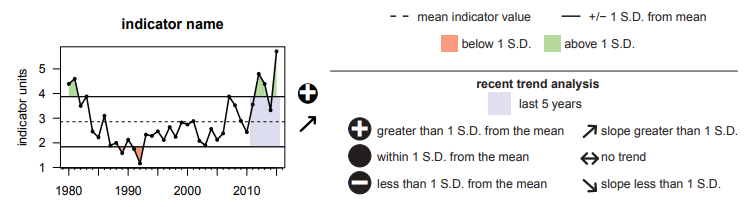
\includegraphics{figures/images/indicator_selection_diagram.png}

}

\caption{\label{fig-explot}Example time series plot, showing an
indicator plotted with its mean and standard deviation, and trend
analysis for the most recent five years of data. See text for a more
detailed description of specific calculations.}

\end{figure}%

\bookmarksetup{startatroot}

\chapter{Tracking performance toward fishery management
objectives}\label{tracking-performance-toward-fishery-management-objectives}

\begin{tcolorbox}[enhanced jigsaw, arc=.35mm, coltitle=black, leftrule=.75mm, titlerule=0mm, bottomrule=.15mm, colback=white, opacitybacktitle=0.6, colframe=quarto-callout-note-color-frame, opacityback=0, rightrule=.15mm, toprule=.15mm, bottomtitle=1mm, toptitle=1mm, title=\textcolor{quarto-callout-note-color}{\faInfo}\hspace{0.5em}{Editing this template page}, breakable, colbacktitle=quarto-callout-note-color!10!white, left=2mm]

Template text is pulled from the 2025 Caribbean Ecosystem Status Report.
Adjust accordingly.

\end{tcolorbox}

In this section, we report indicators that are intended to capture
progress towards meeting Fishery Management Plan objectives related to
food production, socioeconomic health, equity, engagement and
participation, bycatch reduction, governance and protection of
ecosystems.

\bookmarksetup{startatroot}

\chapter{Risks to meeting fishery management
objectives}\label{risks-to-meeting-fishery-management-objectives}

\begin{tcolorbox}[enhanced jigsaw, arc=.35mm, coltitle=black, leftrule=.75mm, titlerule=0mm, bottomrule=.15mm, colback=white, opacitybacktitle=0.6, colframe=quarto-callout-note-color-frame, opacityback=0, rightrule=.15mm, toprule=.15mm, bottomtitle=1mm, toptitle=1mm, title=\textcolor{quarto-callout-note-color}{\faInfo}\hspace{0.5em}{Editing this template page}, breakable, colbacktitle=quarto-callout-note-color!10!white, left=2mm]

Template text is pulled from the 2025 Caribbean Ecosystem Status Report.
Adjust accordingly.

\end{tcolorbox}

In this section, we report indicators that capture identified risks to
the ecosystem that could impact the ability to meet Fishery Management
Plan objectives. Unless otherwise specified, physical indicators
reported for the U.S. Caribbean region were calculated over a bounding
box with limits of longitude 68 degrees W to 64.5 degrees W and latitude
17.5 degrees N to 18.75 degrees N.

\bookmarksetup{startatroot}

\chapter{Integrated ecosystem
perspectives}\label{integrated-ecosystem-perspectives}

\section*{}\label{section}
\addcontentsline{toc}{section}{}

\markright{}

Synthesis

\bookmarksetup{startatroot}

\chapter{Research recommendations}\label{research-recommendations}

Recommendations

\bookmarksetup{startatroot}

\chapter{Acknowledgments}\label{acknowledgments}

\section{Contributions}\label{contributions}

This report would like to acknowledge the efforts and contributions of:

\section{Resources}\label{resources}

This repo and GitHub Action associated with generating this report was
based on the Openscapes tutorial
\href{https://github.com/Openscapes/quarto-website-tutorial}{quarto-website-tutorial}
by Julia Lowndes and Stefanie Butland.

\bookmarksetup{startatroot}

\chapter{Contributors}\label{contributors}

\section{\texorpdfstring{\textbf{Editors}}{Editors}}\label{editors}

xxx

\section{\texorpdfstring{\textbf{Contributors}}{Contributors}}\label{contributors-1}

xxx

\bookmarksetup{startatroot}

\chapter*{References}\label{references}
\addcontentsline{toc}{chapter}{References}

\markboth{References}{References}

\phantomsection\label{refs}
\begin{CSLReferences}{1}{0}
\bibitem[\citeproctext]{ref-MONTENERO2021104489}
Montenero, Kelly, Chris Kelble, and Kathy Broughton. 2021. {``A
Quantitative and Qualitative Decision-Making Process for Selecting
Indicators to Track Ecosystem Condition.''} \emph{Marine Policy} 129:
104489.
https://doi.org/\url{https://doi.org/10.1016/j.marpol.2021.104489}.

\bibitem[\citeproctext]{ref-seara2024}
Seara, Tarsila, Stacey M. Williams, Kiara Acevedo, Graciela
Garcia-Molliner, Orian Tzadik, Michelle Duval, and Juan J. Cruz-Motta.
2024. {``Development and Analyses of Stakeholder Driven Conceptual
Models to Support the Implementation of Ecosystem-Based Fisheries
Management in the U.S. Caribbean.''} \emph{PLOS ONE} 19 (5): e0304101.
\url{https://doi.org/10.1371/journal.pone.0304101}.

\end{CSLReferences}


\backmatter

\end{document}
